\label{sec:singular2}

\todo[inline, color=pink]{Função objetivo}

Seja a seguinte função objetivo:
%
\begin{equation}
	\label{eq:singular2:J}
	J = x_3(t_f)
\end{equation}
%
sujeito ao conjunto de equações diferenciais e restrição no controle:
%
\begin{equation}
	\label{eq:singular2:dinamica}
	\begin{gathered}
		\dot{x}_1(t) = x_2(t),\;\;x_1(0) = 0 \\
		\dot{x}_2(t) = u(t),\;\;x_2(0) = 1 \\
		\dot{x}_3(t) = x_1^2(t) + x_2^2(t),\;\;x_3(0) = 0\\
		-1 \leq |u(t)| \leq 1
	\end{gathered}
\end{equation}
%
em que $t$ é o tempo ($t_f$ é o tempo final) e $ \mathbf{x}(t) = \begin{bmatrix} x_1(t) & x_2(t) & x_3(t) \end{bmatrix}^T $ é o vetor de variáveis de estado e $ u(t) $ é a variável de controle. 

Conforme o primeiro estudo de caso singular, a estimativa inicial para o estado e para o controle foi determinada por cada pacote. 

\todo[inline, color=pink]{Introdução da análise de sensibilidade $ J \times N $}

São apresentados na Figura \ref{fig:singular2:sensibilidade:J} a influência do número de nós de colocação no valor da função objetivo (melhor solução encontrada). A faixa considera nesta análise é a mesma empregada para o problema singular 1 (30 pontos igualmente espaçados no intervalo [5 150]).

\noindent	
\begin{minipage}{\textwidth}
	\vspace{\onelineskip}
	\centering
	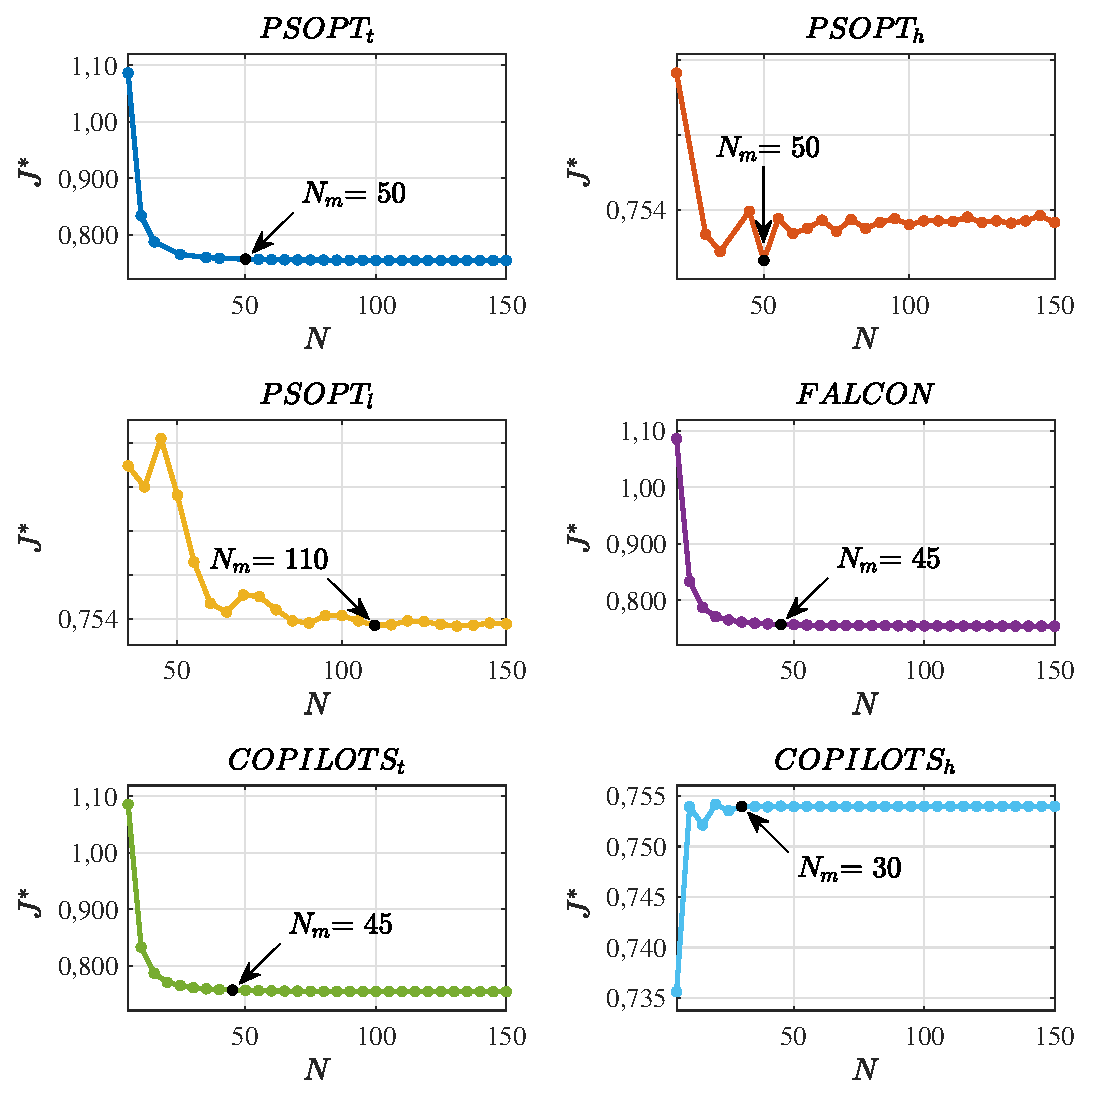
\includegraphics[scale=0.70]{fig/resultados/singular2/sens/J}
	\captionof{figure}[Influência do número de nós de colocação no valor da função objetivo para o problema singular 2]{Influência do número de nós de colocação $ N $ no valor da função objetivo $ J^* $ para o problema singular 2.}
	\label{fig:singular2:sensibilidade:J}
	\vspace{\onelineskip}
\end{minipage}

\todo[inline, color=pink]{Análise dos gráficos $ J \times N $}

De forma geral observa-se que a maioria dos pacotes utilizados, a partir de um determinado valor de $ N_m $, conseguiram convergir para a solução reportada por \textcolor{red}{Arthur, aqui colocar a referência e o valor ótimo para o problema}. O único em que não foi observada uma tendência de convergência ao se aumentar o valor de $N$ foi o $ PSOPT_h$. Para este observa-se um comportamento oscilatório. Assim, o valor de $ N_m $ para esta configuração foi definido como sendo aquele com o menor valor em termos de $ J^* $. Já para o $ COPILOTS_h $ verifica-se um comportamento inesperado, isto é; tanto $ J^* $ quanto $ N $ crescem simultaneamente até que a convergência seja atingida. Tal comportamento pode ser justificado pelo não atendimento das restrições para um número de pontos inferior à, aproximadamente, 30 nós de colocação. Neste caso, por não atender as restrições não considera-se, para $N$ menor que, aproximadamente, 30, que a solução do problema tenha sido obtida. Este resultado inesperado justifica a necessidade de sempre realizar a análise de sensibilidade do problema, bem como avaliar o atendimento das restrições que constituem o mesmo.

\textcolor{red}{Arthur, tentei justificar esse comportamento a partir do não atendimento das restições, mesmo sem saber se é isso. KKKK. Eu imagino que seja isso. O não atendimento pode levar a resultados incoerentes, principalmente no que tange a FO. Por este motivo esta justificativa não é tão groseira ... concorda?}
%sendo 
%%
%\begin{equation}
%J_{N_m} = 0,99 \, \big(max(J^*) - min(J^*)\big) + min(J^*)
%\end{equation}

Além disso, pode ser observada uma boa concordância entre os resultados obtidos por quase todas as abordagens que fazem uso da colocação trapezoidal ($ PSOPT_t $, o $ FALCON $ e o $ COPILOTS_t $). No entanto, observa-se que, empregando o $ PSOPT_t $, não foi possível solucionar o estudo de caso em análise para $ N = 20 $, $ N = 30 $ e $ N = 45 $. Também é possível observar que o valor de $ J^* $ encontrado pelo $ PSOPT_l $ diminui lentamente com o aumento de $ N $ e oscila algumas vezes antes de atingir a convergência. Tal comportamento pode estar associado às propriedades numéricas inerentes à colocação pseudo-espectral, sendo que esta não é a abordagem mais empregada para a  resolução de PCOs com descontinuidades nos controles e/ou estados \cite{becerra_tutorial_2010}. 

Por fim destaca-se que o valor de $ J^* $ referente ao $ PSOPT_h $ se mostrou pouco sensível a variações em $ N $, sendo $ \min(J^*) = 0,753932 $ e $ \max(J^*) = 0,754183$. O mesmo pode ser observado para o $ PSOPT_l $, sendo nesse caso $ \min(J^*) = 0,753984 $ e $\max(J^*) = 0,754411$. 

\todo[inline, color=pink]{Introdução dos resultados $ N = N_m $}

A  Tabela \ref{tab:singular2:raw} apresenta um resumo das métricas obtidas por cada pacote. Neste destacam-se o valor da função objetivo ($ J^* $), o tempo de processamento médio ($ t_p $), o desvio padrão atribuído ($ s_t $), a máxima violação das restrições ($ \Delta c_{max} $) e o número de execuções bem sucedidas ($ N_s $).

\begin{table}[!h]
	\centering
	\caption[Métricas obtidas para o problema singular 2]{Métricas obtidas para o problema singular 2. Os melhores $ N_m $, $ J^* $, $ t_p $, $ n_{aval} $ e $ N_s\% $ se encontram destacados.}
	\label{tab:singular2:raw}
	\begin{tabular}{ccccccccc}
		\hline
		Método       & $N_m$                              & $J^*$                                   & $t_p$ {[}$s${]}                         & $s_t$ {[}$s${]} & $n_{aval}$                         & $\Delta c_{max}$                & $N_s$ & $N_s\%$                                  \\ \hline
		$PSOPT_t$    & 50                                 & 0,75663                                 & 3,20295                                 & 0,08123         & 924                                & 3,12e-11                        & 27    & 90,00\%                                  \\
		$PSOPT_h$    & 50                                 & {\color[HTML]{009901} \textbf{0,75393}} & 3,50511                                 & 0,08317         & 1060                               & 4,16e-09                        & 25    & 83,33\%                                  \\
		$PSOPT_l$    & 110                                & 0,75399                                 & 15,91228                                & 0,16007         & 214                                & 1,16e-07                        & 24    & 80,00\%                                  \\
		$FALCON$     & 45                                 & 0,75720                                 & {\color[HTML]{009901} \textbf{0,37631}} & 0,04386         & {\color[HTML]{009901} \textbf{76}} & 2,36e-09                        & 30    & {\color[HTML]{009901} \textbf{100,00\%}} \\
		$COPILOTS_t$ & 45                                 & 0,75720                                 & 17,77565                                & 0,37422         & 37149                              & 3,32e-12                        & 30    & {\color[HTML]{009901} \textbf{100,00\%}} \\
		$COPILOTS_h$ & {\color[HTML]{009901} \textbf{30}} & 0,75397                                 & 34,27460                                & 0,41814         & 105399                             & {\color[HTML]{000000} 1,63e-12} & 30    & {\color[HTML]{009901} \textbf{100,00\%}} \\ \hline
	\end{tabular}
\end{table}

\todo[inline, color=pink]{Análise dos resultados $ N = N_m $}

Nesta tabela, os valores de $ J^* $ associados ao $ PSOPT_h $ e ao $ COPILOTS_h $ se mostram bastante próximos, sendo o $ J^* $ atribuído ao $ PSOPT_h $ o menor dentre os obtidos. Em relação ao $ FALCON $ e ao $ COPILOTS $, associam-se os menores $ N_m $. Além disso, observa-se no $ COPILOTS_h $ o menor valor em termos de $ N_m $. Em geral, os $ N_m $ associados aos métodos que fazem uso da colocação trapezoidal são maiores que os requeridos pelos que empregam a colocação de  Hermite-Simson. De fato, essa tendência é observada quando comparam-se os valores de $ N_m $ do $ COPILOTS_t $ e do $ COPILOTS_h $. No entanto, não se verifica esse mesmo comportamento quando avaliam-se os $ N_m $ associados ao $ PSOPT_t $ e ao $ PSOPT_h $. Esse resultado pode estar relacionado ao tipo de otimizador considerado pelo  $ PSOPT $, isto é. ao Método de Ponto Interior \cite{wachter_implementation_2006}.

Ao se empregar o $ FALCON $ observa-se os menores valores para $ t_p $ e para $ n_{aval} $. Em contrapartida, ao $ COPILOTS $ estão associados os maiores $ t_p $ e $ n_{aval} $. Provavelmente, esta diferença se deve as características de cada pacote, bem como ao uso de informações simbólicas empregadas pelo $ FALCON $. Foi somente empregando o $ COPILOTS $ e o $ FALCON $ que este estudo de caso foi resolvido para os valores de $N$ adotados. Por outro lado, o menor valor de $ N\% $ e o maior valor de $ N_m $ foi obtido pelo $ PSOPT_l $. Esses resultados indicam que a colocação pseudo-espectral não deve ser empregada na resolução de PCOs aos quais estejam associadas descontinuidades nos controles e/ou estados \cite{becerra_tutorial_2010}. 

É importante ressaltar que em relação ao $ PSOPT $, o maior valor de $ t_p $ foi encontrado para a configuração pseudo-espectral. Esse resultado indica que nem sempre há uma relação direta entre $ t_p $ e $ n_{aval} $, e que a associação entre essas variáveis depende do método empregado na resolução do estudo de caso em análise. 

\todo[inline, color=pink]{Introdução das trajetórias}

As trajetórias obtidas para o vetor de variáveis de estado e controle são apresentadas nas Figuras \ref{fig:singular2:x:x1}-\ref{fig:singular2:u:u} considerando $N$ igual a $N_m$. Ao se analisar os resultados pode-se perceber a similaridade entre todos os perfis referentes as variáveis de estado. Em relação ao controle, observa-se uma mesma tendência, todavia são observadas oscilações na maiores dos pacotes. As trajetórias de controle associadas ao $ PSOPT_t $ e ao $ PSOPT_h $ se mostraram oscilatórias, o que pode ser devido ao otimizador considerado. Já aquelas associadas aos demais métodos apresentaram apenas leves oscilações após a primeira variação abrupta de $ u(t) $, que ocorre em $ t \approx 1,3 $ s. No caso do $ PSOPT_l $ foram observadas leves oscilações ao fim da trajetória, o que se deve ao alto valor de $ N_m $ empregado. Em contrapartida, o $ FALCON $ apresenta uma trajetória mais suave em relação as outras abordagens empregadas. 

A influência do número de nós de colocação no tempo de processamento e no número de avaliações da função objetivo são apresentadas nas Figuras \ref{fig:singular2:sensibilidade:t} e \ref{fig:singular2:sensibilidade:naval}. Nestes gráficos são apresentadas as variações: $ \Delta t_p = \max\{t_p\} - \min\{t_p\} $ e $ \Delta n_{aval} = \max\{n_{aval}\} - \min\{n_{aval}\} $. Os pontos nos gráficos representam os valores atribuídos a $ t_p $ (e a $ n_{aval} $) para cada um dos $ N $ considerados, enquanto as linhas contínuas representam curvas de tendência, obtidas por meio de regressões lineares, em que $R^2$ é o coeficiente de determinação. Os valores de $ N $ empregados na geração desses resultados são iguais àqueles considerados na computação da relação entre $ J^* $ e $ N $. 

\noindent
\begin{minipage}{\textwidth}
	\vspace{\onelineskip}
	\centering
	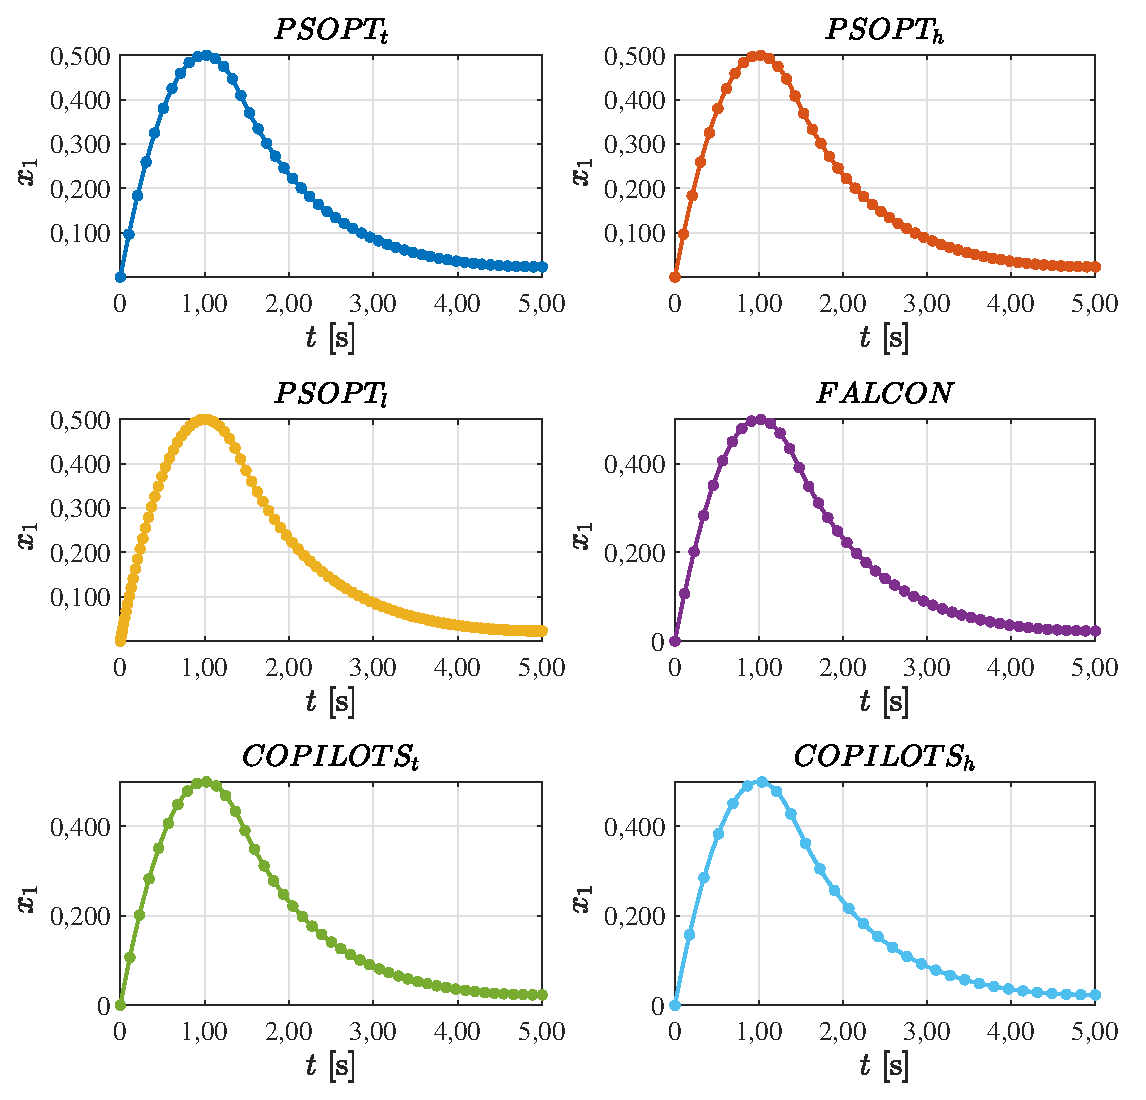
\includegraphics[scale=0.70]{fig/resultados/singular2/traj/x/x_1}
	\captionof{figure}[	Variável de estado $x_1(t)$ para o problema singular 2]{Variável de estado $x_1(t)$ para o problema singular 2. Os pontos representam os valores discretizados e as linhas contínuas representam as trajetórias interpoladas.}
	\label{fig:singular2:x:x1}
	\vspace{\onelineskip}
\end{minipage}

\noindent
\begin{minipage}{\textwidth}
	\vspace{\onelineskip}
	\centering
	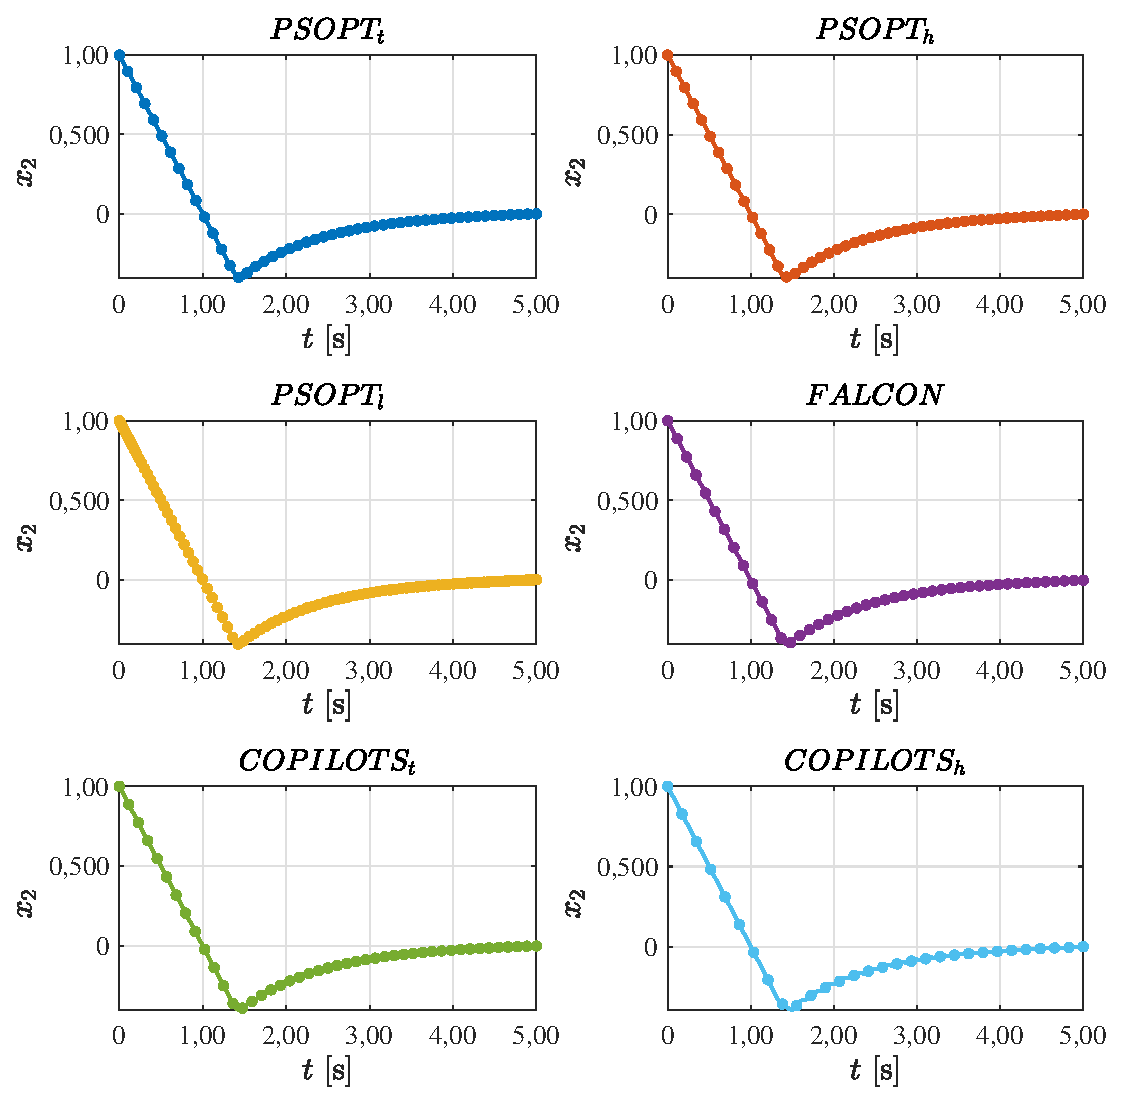
\includegraphics[scale=0.70]{fig/resultados/singular2/traj/x/x_2}
	\captionof{figure}[Variável de estado $x_2(t)$ para o problema singular 2]{Variável de estado $x_2(t)$ para o problema singular 2. Os pontos representam os valores discretizados e as linhas contínuas representam as trajetórias interpoladas.}
	\label{fig:singular2:x:x2}
	\vspace{\onelineskip}
\end{minipage}

\noindent
\begin{minipage}{\textwidth}
	\vspace{\onelineskip}
	\centering
	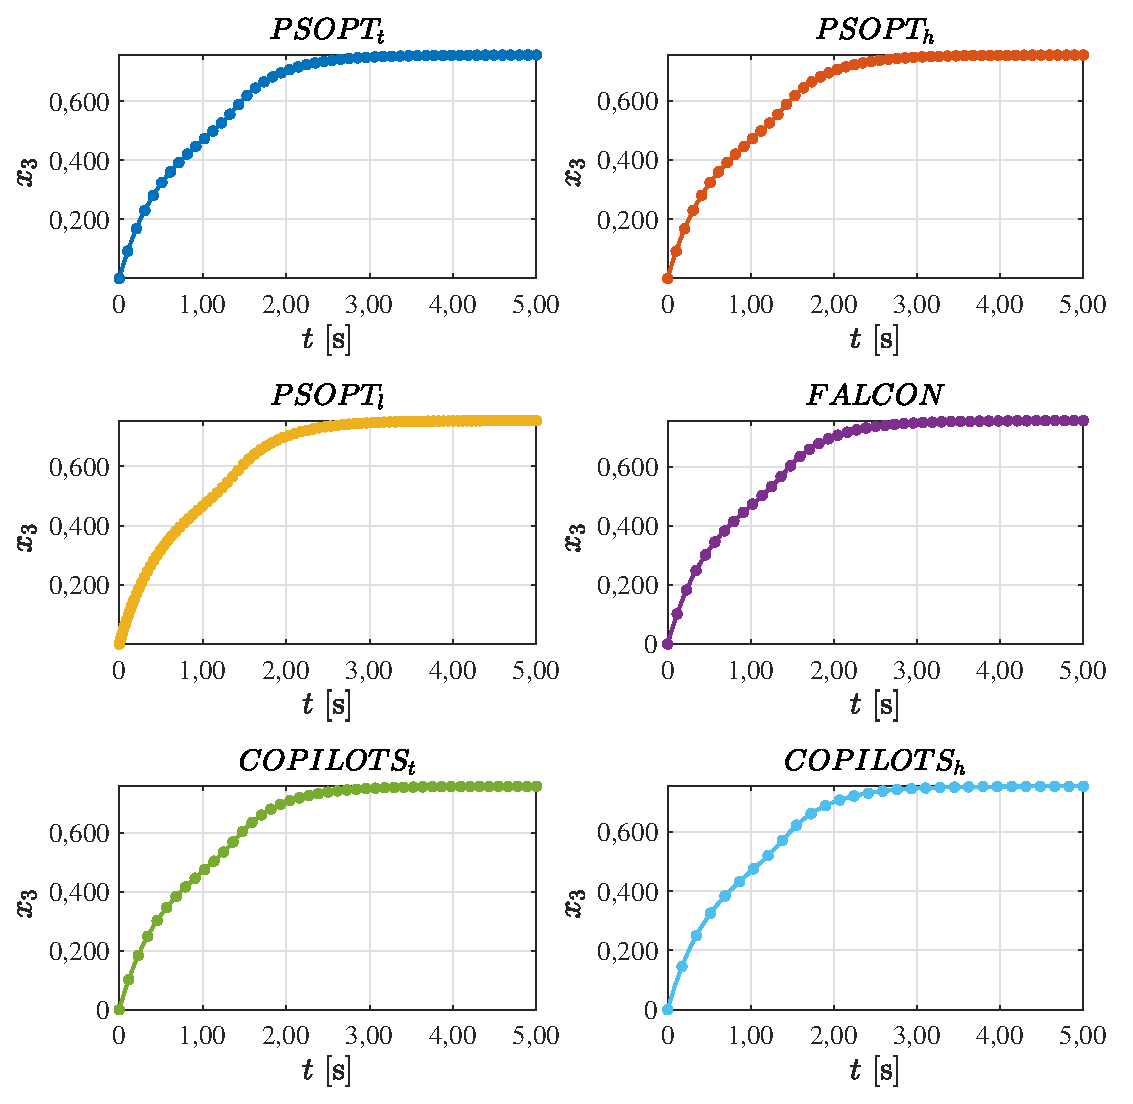
\includegraphics[scale=0.70]{fig/resultados/singular2/traj/x/x_3}
	\captionof{figure}[Variável de estado $x_3(t)$ para o problema singular 2]{Variável de estado $x_3(t)$ para o problema singular 2. Os pontos representam os valores discretizados e as linhas contínuas representam as trajetórias interpoladas.}
	\label{fig:singular2:x:x3}
	\vspace{\onelineskip}
\end{minipage}

\noindent
\begin{minipage}{\textwidth}
	\vspace{\onelineskip}
	\centering
	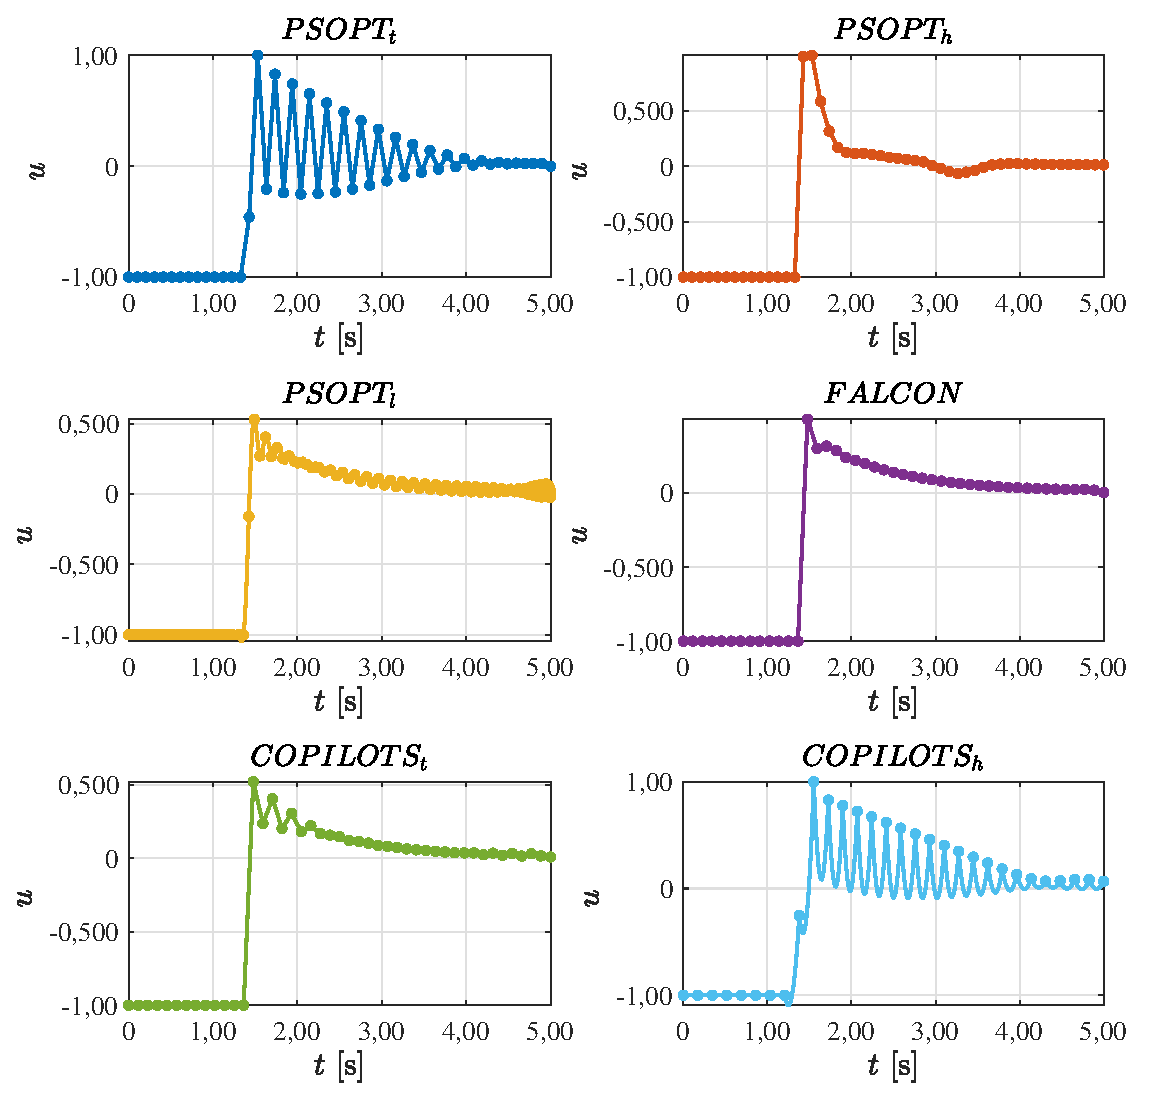
\includegraphics[scale=0.70]{fig/resultados/singular2/traj/u/u}
	\captionof{figure}[Variável de controle $u(t)$ para o problema singular 2]{Variável de controle $u(t)$ para o problema singular 2. Os pontos representam os valores discretizados e as linhas contínuas representam as trajetórias interpoladas.}
	\label{fig:singular2:u:u}
	\vspace{\onelineskip}
\end{minipage}

\todo[inline, color=pink]{Análise das trajetórias}


\todo[inline, color=pink]{Introdução dos resultados $ t_p \times N $ e $ n_{aval} \times N $}

\noindent
\begin{minipage}{\textwidth}
	\vspace{\onelineskip}
	\centering
	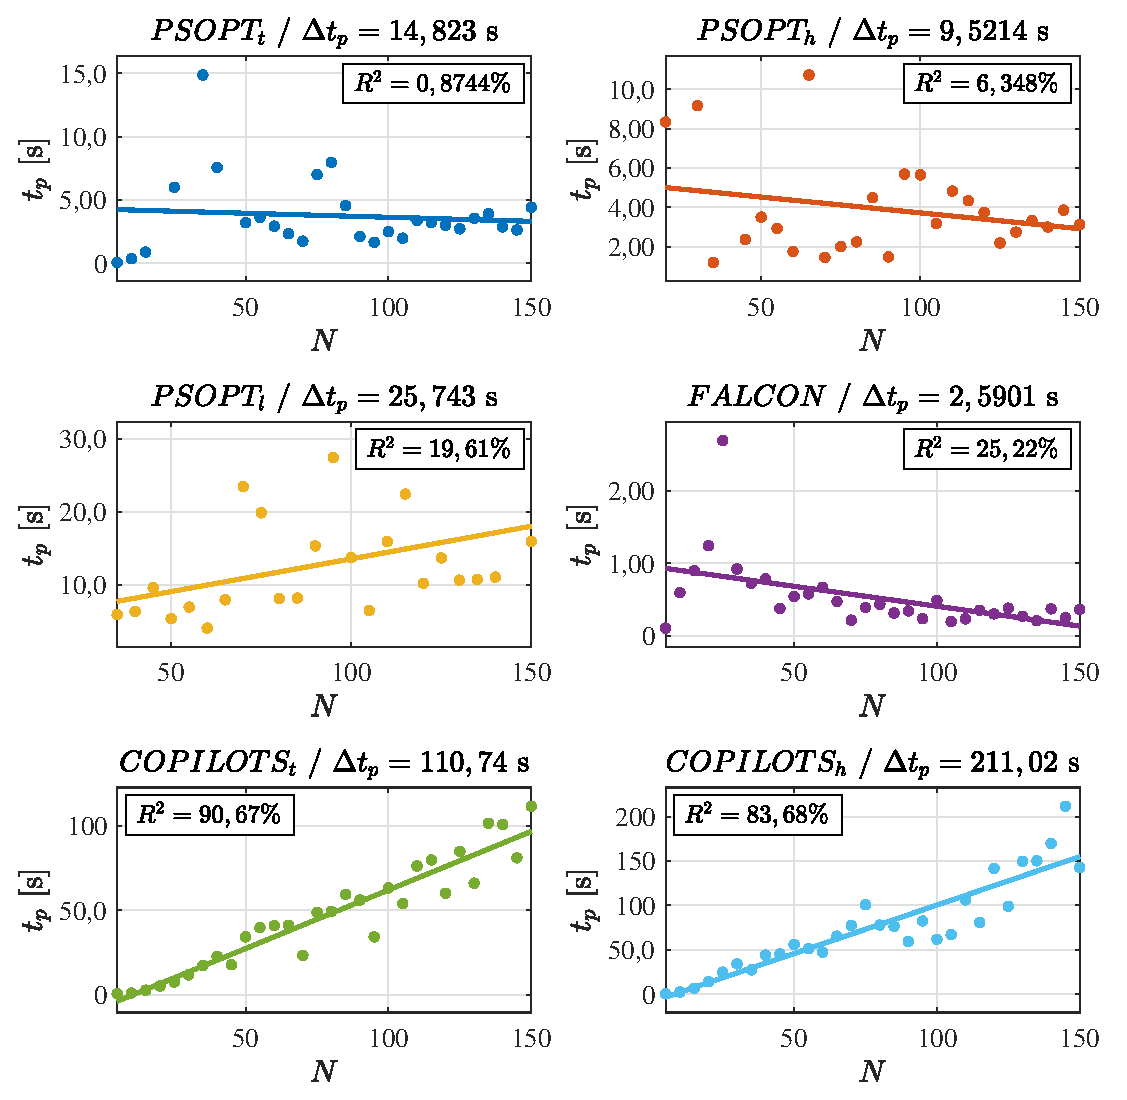
\includegraphics[scale=0.70]{fig/resultados/singular2/sens/t}
	\captionof{figure}[Relação entre o tempo de processamento e o número de nós de colocação para o problema singular 2]{Relação entre o tempo de processamento $ t_p $ e o número de nós de colocação $ N $, considerando cada um dos métodos em análise.}
	\label{fig:singular2:sensibilidade:t}
	\vspace{\onelineskip}
\end{minipage}

Nas Figuras \ref{fig:singular2:sensibilidade:t} e \ref{fig:singular2:sensibilidade:naval} observa-se que os valores de $ t_p $ e de $ n_{aval} $ associados ao $ FALCON $ se mostraram pouco sensíveis a variações em $ N $, dados os baixos $ \Delta t_p $ e $ \Delta n_{aval} $ associados a esse pacote. Em relação ao $ PSOPT$, a configuração pseudo-espectral foi a que resultou em um maior tempo de processamento. Esse comportamento se deve às características numéricas inerentes à colocação pseudo-espectral, que não deve ser empregada na solução de PCOs aos quais estejam associadas descontinuidades nos controles \cite{becerra_tutorial_2010}. Em contrapartida, o $ n_{aval} $ vinculado ao $ PSOPT_l $ se mostrou menos sensível a variações em $ N $ que aqueles associados ao $ PSOPT_t $ e ao $ PSOPT_h $. 

Os métodos associados ao $ COPILOTS $ se mostraram bastante sensíveis a variações em $ N $, com $ \Delta t_p $ e $ \Delta n_{aval} $ consideravelmente mais altos que os atribuídos aos demais métodos. Esse comportamento se deve ao uso que o pacote faz do SQP utilzado. Com o aumento de $ N $, os valores de $ t_p $ e de $ n_{aval} $ associados ao $ PSOPT_t $, $ PSOPT_h $ e $ FALCON $, e os valores de $ n_{aval} $ requeridos pelo $ PSOPT_l $ tendem a convergir. Além disso, nota-se que os valores de $ t_p $ e de $ n_{aval} $ diminuem à medida que alcançam essa convergência para algumas configurações utilizadas, comportamento oposto àquele que espera-se observar nesses casos. A presença de picos nos $ t_p $ e $ n_{aval} $ observados em cada um desses métodos ajuda a explicar este comportamento anômalo. Em resumo, devido à presença de alguns picos existe uma falsa impressão que o aumento no valor de $N$ implica na redução do tempo de processamento (ver a Figura \ref{fig:singular2:sensibilidade:t}). Este mesmo comportamento pode ser observado na Figura \ref{fig:singular2:sensibilidade:naval} para todas as configurações $ PSOPT$ e do $FALCON $. Neste caso, menores valores de $N$ podem resultar em um menor número de avaliações da função objetivo, porém, a convergência acontece para um valor que não é a solução do problema, conforme observado na Figura \ref{fig:singular2:sensibilidade:J}. Já para todas as versões do $ COPILOTS $ são observados perfis mais próximos aos esperados para $ t_p $ e de $ n_{aval} $, isto é; o aumento no valor de $N$ implica no aumento destes dois parâmetros, conforme observado nas Figuras \ref{fig:singular2:sensibilidade:t}) e  \ref{fig:singular2:sensibilidade:naval}.

\noindent
\begin{minipage}{\textwidth}
	\vspace{\onelineskip}
	\centering
	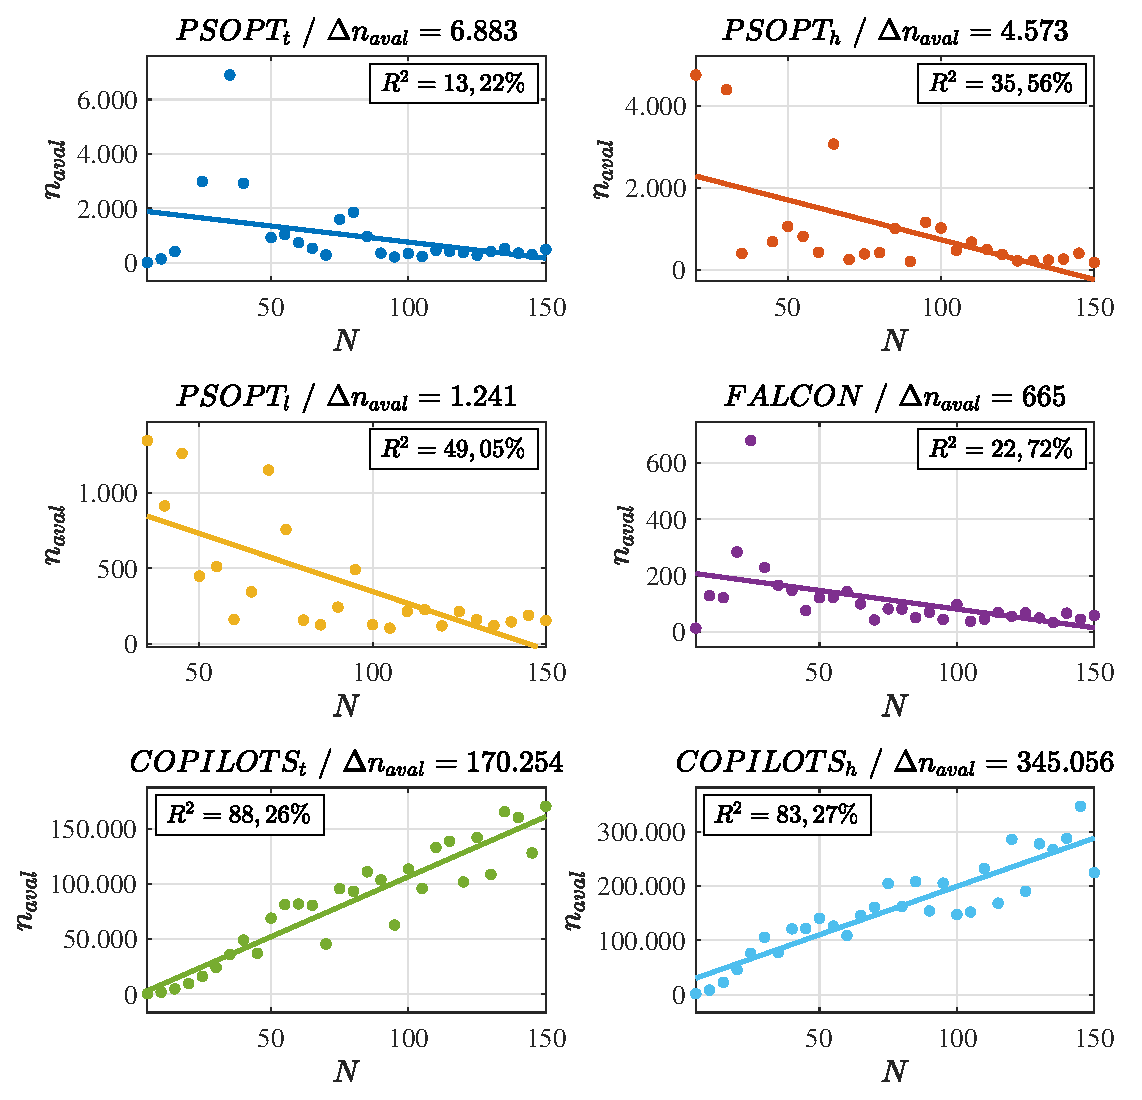
\includegraphics[scale=0.70]{fig/resultados/singular2/sens/eval}
	\captionof{figure}[Relação entre o número de avaliações da função objetivo e o número de nós de colocação para o problema singular 2]{Relação entre o número de avaliações da função objetivo $ n_{aval} $ e o número de nós de colocação $ N $, considerando cada um dos métodos em análise.}
	\label{fig:singular2:sensibilidade:naval}
	\vspace{\onelineskip}
\end{minipage}

\todo[inline, color=pink]{Análise dos resultados $ t_p \times N $ e $ n_{aval} \times N $}

